
\documentclass[acmsmall,screen]{acmart}

\setcopyright{none}
\settopmatter{printacmref=false}
\renewcommand\footnotetextcopyrightpermission[1]{}
\acmJournal{CSUR}

\usepackage{booktabs}
\usepackage{tabularx}
\usepackage{multirow}
\usepackage{amsmath,amssymb}
\usepackage{tikz}
\usetikzlibrary{arrows.meta,positioning,shapes.geometric}
\usepackage{enumitem}
\usepackage{microtype}

\title{Benchmarking AutoML and Agentic Pipelines Against Expert-Tuned Models on Small Datasets}
\subtitle{A Literature-Grounded Review and Benchmarking Framework for Small-Data Tabular Machine Learning}

\author{Rachna Gupta}
\authornote{Roll No.: rsi2026510; Topic ID: 27}
\affiliation{\institution{AI Tools for Research}\city{Prayagraj}\country{India}}

\begin{abstract}
Small tabular datasets provide a difficult machine-learning regime because limited observations raise estimator variance, heighten sensitivity to preprocessing and hyperparameter choices, and make standard train/validation/test divisions statistically brittle. At the same time, automated machine learning (AutoML) has progressed from automatic hyperparameter optimisation to systems capable of model selection, feature preprocessing, ensembling, and more self-contained pipeline design. Agentic systems based on large language models (LLMs) present a new paradigm in which autonomous or multi-agent systems organise, implement, execute, evaluate, and adjust machine-learning processes. This study looks at existing research on standard AutoML, machine-learning models for short datasets, and agentic ML systems, with a focus on how these approaches might be reasonably compared to expert-tuned models. The literature is divided into four categories: expert-designed pipelines, traditional AutoML frameworks, LLM-based agentic systems, and models created specifically for tiny datasets. Previous research indicates that predicted accuracy alone does not provide a clear picture of their usefulness. Validation methodologies, computing resources, model stability, calibration, reproducibility, interpretability, and human involvement are all factors that influence the outcomes. However, very few research have investigated all four techniques under consistent experimental settings. To close this gap, the proposed benchmark uses a standard evaluation process that includes stringent data separation, nested validation, comparable computing budgets, repeated tests, and numerous performance measurements.



% This review synthesizes literature on conventional AutoML, small-data-specific models, and agentic machine-learning systems, with emphasis on the methodological conditions required for a fair comparison with expert-tuned models. The review organizes the literature around four methodological families: expert-tuned pipelines, conventional AutoML, LLM-driven agentic pipelines, and specialized small-data foundation models. Across these families, predictive performance alone is insufficient for comparison. Validation design, search-space definition, computational cost, stability, calibration, reproducibility, interpretability, and human effort materially affect conclusions. The central gap is the limited availability of controlled studies that compare strong expert baselines, conventional AutoML, agentic systems, and small-data-specific models under the same small-data protocol. A literature-grounded benchmark is therefore proposed using strict information boundaries, nested validation, controlled compute budgets, repeated resampling, and multi-dimensional evaluation.
\end{abstract}

\keywords{Automated Machine Learning, AutoML, Agentic AI, LLM Agents, Small Data, Tabular Machine Learning, Hyperparameter Optimization, Benchmarking, Expert Tuning, TabPFN}

\begin{document}
\maketitle

\section{Introduction}\label{sec:intro}

% Machine learning practice traditionally combines algorithmic methods with human decisions about preprocessing, feature engineering, validation, model families, hyperparameters, error analysis, and final model selection. Automated machine learning (AutoML) emerged partly to reduce this manual burden by automating model selection, hyperparameter optimization, preprocessing, feature selection, and pipeline construction \cite{feurer2015,olson2016}. The resulting systems changed the role of the practitioner from repeatedly implementing individual experiments toward defining search spaces, budgets, and evaluation protocols.

% Early AutoML systems framed development as a structured optimization problem. Auto-sklearn combined Bayesian optimization, meta-learning, and ensemble construction \cite{feurer2015}, while TPOT used genetic programming to search over machine-learning pipelines \cite{olson2016}. Later methods introduced resource-aware search, including Hyperband \cite{li2018} and BOHB \cite{falkner2018}, while FLAML emphasized efficient search under constrained budgets \cite{wang2021}. AutoGluon-Tabular emphasized model diversity, stacking, and multi-layer ensembles \cite{erickson2020}.

In classical machine learning, the practitioner must make multiple decisions before constructing a solid model, including data preprocessing, feature engineering, validation, algorithm selection, hyperparameter tuning, and performance analysis. Automated machine learning (AutoML) streamlines model building by automating algorithm selection, hyperparameter optimization, feature selection, and pipeline design \cite{feurer2015,olson2016}. Instead of performing each experiment manually, practitioners can use these tools to focus on identifying appropriate search spaces, defining computational constraints, and devising assessment processes.


Early AutoML frameworks approached model development as an optimization task. To find appropriate models, Auto-sklearn used ensemble techniques, meta-learning, and Bayesian optimisation \cite{feurer2015}. In contrast, TPOT used genetic programming to investigate various combinations of learning algorithms and preprocessing methods \cite{olson2016}. Later methods concentrated on increasing the effectiveness of searches and the usage of resources. While FLAML sought to attain competitive performance with constrained computational budgets \cite{wang2021}, Hyperband \cite{li2018} and BOHB \cite{falkner2018} introduced techniques for allocating computational resources during hyperparameter search. A alternative approach was used by AutoGluon-Tabular, which combined various models using multi-layer ensembles and stacking \cite{erickson2020}.

Working with small datasets introduces additional challenges in model development and evaluation. When only a limited number of samples are available, setting aside data for validation reduces the amount available for training. Testing numerous model configurations on the same validation set may also lead to unreliable model selection because the results can be influenced by random variations in the data. Running more experiments does not necessarily improve the quality of the available evidence. Therefore, a reliable comparison should consider both the model optimization process and the statistical confidence of the validation results.

Another method for automating machine-learning tasks has been presented by the increasing use of large language models (LLMs). LLM-based agents are able to analyse datasets, develop and run code, find mistakes, provide preparation techniques, and adjust their processes in response to experimental findings. For example, AutoML-Agent automates entire machine-learning pipelines by combining numerous verification phases, retrieval-augmented planning, and specialised agents \cite{trirat2025}. These systems have the ability to decide how the entire workflow should be structured, in contrast to traditional AutoML techniques that mostly investigate established settings.

In the meanwhile, a substitute for extensive model searching is provided by models built for limited datasets. With little hyperparameter tuning, TabPFN has shown competitive prediction performance in classification tasks involving tiny tabular datasets by using a pretrained Transformer \cite{hollmann2023}. These strategies imply that no single solution is likely to work optimally in every circumstance. The qualities of the dataset, the computational resources at hand, the validation processes, and the availability of pertinent data all influence how valuable they are.

Four primary goals are addressed in this review. Using a uniform set of evaluation criteria, it initially divides current approaches into four methodological categories before analysing their benefits and drawbacks. Additionally, it addresses problems such validation overfitting, search-space bias, data leakage, inconsistent results between runs, and variations in computing budgets that could compromise the reliability of comparisons. Lastly, it describes a controlled benchmarking process for comparing similar experimental settings between expert-tuned models, traditional AutoML frameworks, LLM-based agentic systems, and specialised small-data models.



% The small-data setting changes the methodological question. When the number of observations is limited, a validation split consumes a relatively large fraction of available information. Repeatedly evaluating many configurations on the same validation data can also make the selection process sensitive to validation noise. Thus, the ability to run more experiments does not itself create more statistical information. A fair comparison must separate the optimization procedure from the statistical reliability of the evidence used to choose a model.

% The question becomes more complex with large language models (LLMs). LLM-based agents can inspect data, generate code, interpret errors, propose preprocessing, execute experiments, and revise their own workflow. AutoML-Agent, for example, uses multiple specialized agents, retrieval-augmented planning, and multi-stage verification for full-pipeline AutoML \cite{trirat2025}. This expands the optimization target from a predefined configuration space toward workflow design itself.

% At the same time, specialized small-data models challenge the assumption that extensive search is always necessary. TabPFN uses a pretrained Transformer for small tabular classification and reports competitive performance with very low tuning cost \cite{hollmann2023}. These developments motivate a review that does not assume a universal winner. Instead, the relevant question is under what data, budget, validation, and information-access conditions each methodological family is useful.

% This paper makes four review-level contributions. First, it develops a taxonomy of four methodological families. Second, it synthesizes their strengths and limitations using common evaluation dimensions. Third, it identifies methodological threats that can make comparisons misleading, especially validation overfitting, search-space bias, leakage, nondeterminism, and unequal computational budgets. Fourth, it proposes a controlled benchmark protocol for comparing expert-tuned, conventional AutoML, agentic, and specialized small-data approaches.

\section{Review Scope and Methodological Framing}\label{sec:scope}



The literature considered in this review addresses a common problem: how can automated machine-learning methods be compared fairly with expert-designed approaches when only a small amount of tabular data is available? To examine this question, we consider studies covering early AutoML frameworks, hyperparameter search, benchmarking practices, models developed for small datasets, and recent LLM-based agentic systems \cite{hutter2011,feurer2015,olson2016,li2018,falkner2018,erickson2020,wang2021,gijsbers2024,hollmann2023,trirat2025}.

In this study, ``small data'' refers to datasets with limited training observations rather than a fixed definition of dataset complexity. We use the following practical threshold to identify the small-data setting:
\begin{equation}
n_{\mathrm{train}}\leq 1000,
\label{eq:small}
\end{equation}
However, the number of samples alone cannot indicate how difficult a learning task will be. Other characteristics, including the number of features, class distribution, missing values, and noise, can also influence model performance and the reliability of evaluation results.

To describe the relationship between dataset size and dimensionality, we consider
\begin{equation}
\rho=\frac{p}{n},
\label{eq:rho}
\end{equation}
where $p$ represents the number of input features and $n$ denotes the number of training observations. This ratio helps distinguish datasets that contain similar numbers of samples but differ considerably in feature dimensionality.

\subsection{Review Dimensions}

To compare the methods discussed in the literature, eight evaluation aspects are considered:

\begin{enumerate}[leftmargin=*]
\item predictive performance;
\item robustness and stability across repeated evaluations;
\item computational requirements and monetary cost;
\item prediction calibration and statistical validity;
\item model interpretability and auditability;
\item complexity of the resulting pipeline;
\item reproducibility of experimental results; and
\item human effort involved in model development.
\end{enumerate}

These features mirror those brought up in earlier AutoML benchmarking studies \cite{gijsbers2024}, namely the requirement to look at practical costs and evaluation circumstances in addition to predicting performance. When evaluating models meant for limited datasets and workflows run by LLM-based agents, they are also pertinent.

\section{Taxonomy of Approaches}\label{sec:taxonomy}

The four sets of approaches taken into consideration in this review are shown in Figure~\ref{fig:taxonomy}. Although some approaches may have traits in common with more than one category, the grouping is meant to facilitate comparison.

\begin{figure}[t]
\centering
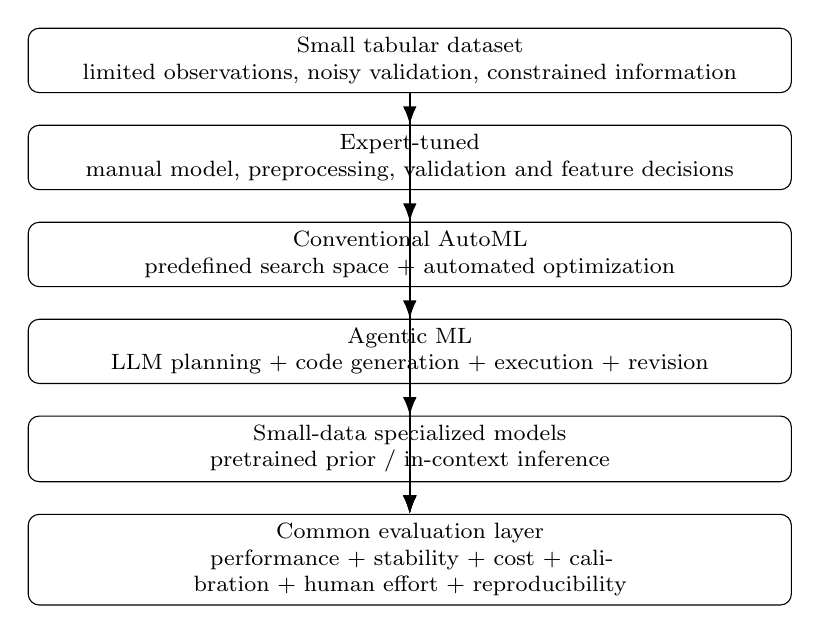
\begin{tikzpicture}[
node distance=4mm and 5mm,
box/.style={draw, rounded corners, align=center, font=\footnotesize, minimum height=8mm, text width=0.78\linewidth},
arrow/.style={-Latex, thick}
]
\node[box] (problem) {Small tabular dataset\\limited observations, noisy validation, constrained information};
\node[box, below=of problem] (expert) {Expert-tuned\\manual model, preprocessing, validation and feature decisions};
\node[box, below=of expert] (automl) {Conventional AutoML\\predefined search space + automated optimization};
\node[box, below=of automl] (agent) {Agentic ML\\LLM planning + code generation + execution + revision};
\node[box, below=of agent] (special) {Small-data specialized models\\pretrained prior / in-context inference};
\node[box, below=of special] (eval) {Common evaluation layer\\performance + stability + cost + calibration + human effort + reproducibility};
\draw[arrow] (problem) -- (expert);
\draw[arrow] (problem) -- (automl);
\draw[arrow] (problem) -- (agent);
\draw[arrow] (problem) -- (special);
\draw[arrow] (expert) -- (eval);
\draw[arrow] (automl) -- (eval);
\draw[arrow] (agent) -- (eval);
\draw[arrow] (special) -- (eval);
\end{tikzpicture}
\caption{Classification of approaches considered for small-data tabular machine-learning comparisons.}
\label{fig:taxonomy}
\Description{A taxonomy connecting small tabular datasets with four groups of machine-learning approaches and a shared evaluation framework.}
\end{figure}

\subsection{Expert-Tuned Models}

The practitioner makes choices about data preparation, feature selection, learning algorithms, hyperparameter settings, and validation techniques in expert-tuned machine learning. These choices are frequently influenced by prior experience and application domain expertise. An experienced practitioner might, for example, select a more appropriate assessment metric for an imbalanced dataset or steer clear of overly complicated models when training samples are scarce. When crucial aspects of the issue are difficult to capture in an automated search process, this flexibility is helpful.

However, the practitioner's time, technical expertise, and personal preferences also play a role in the development of manual models. When the number of viable combinations increases, even seasoned researchers may miss beneficial arrangements. The time spent on model building, the knowledge provided to each method, and the resources consumed during experimentation should therefore be taken into consideration when comparing expert-tuned versus automated approaches.

\subsection{Conventional AutoML}

By searching through a predetermined set of algorithms, preprocessing techniques, and hyperparameter values, conventional AutoML systems minimise manual experimentation. Their primary advantage is the capacity to assess numerous possible configurations via a methodical search process. While TPOT employs genetic programming to find appropriate machine-learning pipelines \cite{olson2016}, Auto-sklearn uses Bayesian optimisation, meta-learning, and ensemble creation \cite{feurer2015}. By distributing resources based on candidate configurations' performance, Hyperband increases search efficiency \cite{li2018}. BOHB combines Bayesian optimization with Hyperband-style resource allocation \cite{falkner2018}, while FLAML focuses on finding effective configurations with limited computational resources \cite{wang2021}.

Despite these advantages, AutoML performance depends heavily on the choices included in its search space. A system cannot select an algorithm or preprocessing method that has not been made available during configuration. Its effectiveness therefore depends not only on the search algorithm but also on the dataset, available model choices, and computational budget.



% The reviewed literature is organized around a common question: how should automated and expert-driven approaches be compared when the available tabular dataset is small? The source literature covers foundational AutoML, hyperparameter optimization, benchmarking, small-data-specific modeling, and LLM-based agentic automation \cite{hutter2011,feurer2015,olson2016,li2018,falkner2018,erickson2020,wang2021,gijsbers2024,hollmann2023,trirat2025}.

% For this review, ``small data'' is treated as an operational research regime rather than a rhetorical label. A practical starting criterion is
% \begin{equation}
% n_{\mathrm{train}}\leq 1000,
% \label{eq:small}
% \end{equation}
% while recognizing that sample size alone does not characterize difficulty. Feature dimensionality, class imbalance, missingness, noise, and feature-to-observation ratio can substantially alter the statistical problem.

% A useful descriptor is
% \begin{equation}
% \rho=\frac{p}{n},
% \label{eq:rho}
% \end{equation}
% where $p$ is the number of features and $n$ is the number of training observations. Equation~\ref{eq:rho} captures an important distinction: two datasets with the same number of observations may have very different levels of dimensional pressure.

% \subsection{Review Dimensions}

% The literature is synthesized using eight dimensions:

% \begin{enumerate}[leftmargin=*]
% \item predictive performance;
% \item robustness and stability under resampling;
% \item computational and monetary cost;
% \item calibration and statistical validity;
% \item interpretability and auditability;
% \item pipeline complexity;
% \item reproducibility; and
% \item human effort.
% \end{enumerate}

% This multidimensional framing follows the methodological concerns emphasized by AutoML benchmarking work \cite{gijsbers2024} and by the small-data and agentic literature reviewed in the source paper.

% \section{Taxonomy of Approaches}\label{sec:taxonomy}

% Figure~\ref{fig:taxonomy} organizes the literature into four methodological families. The taxonomy is analytical rather than a claim that the categories are mutually exclusive in implementation.

% \begin{figure}[t]
% \centering
% \begin{tikzpicture}[
% node distance=4mm and 5mm,
% box/.style={draw, rounded corners, align=center, font=\footnotesize, minimum height=8mm, text width=0.78\linewidth},
% arrow/.style={-Latex, thick}
% ]
% \node[box] (problem) {Small tabular dataset\\limited observations, noisy validation, constrained information};
% \node[box, below=of problem] (expert) {Expert-tuned\\manual model, preprocessing, validation and feature decisions};
% \node[box, below=of expert] (automl) {Conventional AutoML\\predefined search space + automated optimization};
% \node[box, below=of automl] (agent) {Agentic ML\\LLM planning + code generation + execution + revision};
% \node[box, below=of agent] (special) {Small-data specialized models\\pretrained prior / in-context inference};
% \node[box, below=of special] (eval) {Common evaluation layer\\performance + stability + cost + calibration + human effort + reproducibility};
% \draw[arrow] (problem) -- (expert);
% \draw[arrow] (problem) -- (automl);
% \draw[arrow] (problem) -- (agent);
% \draw[arrow] (problem) -- (special);
% \draw[arrow] (expert) -- (eval);
% \draw[arrow] (automl) -- (eval);
% \draw[arrow] (agent) -- (eval);
% \draw[arrow] (special) -- (eval);
% \end{tikzpicture}
% \caption{Literature-grounded taxonomy for comparing methodological families in small-data tabular machine learning.}
% \label{fig:taxonomy}
% \Description{A vertical taxonomy showing a small tabular dataset feeding four methodological families and a common multidimensional evaluation layer.}
% \end{figure}

% \subsection{Expert-Tuned Models}

% Expert tuning uses human knowledge to select preprocessing, candidate algorithms, hyperparameter ranges, validation procedures, feature engineering, and final models. The advantage is that domain knowledge can be applied even when it is difficult to encode in a generic search space. An expert can, for example, recognize when a high-capacity model is inappropriate for the sample size or when class imbalance makes raw accuracy misleading.

% The limitation is that expert search is constrained by time, experience, preferences, and human bias. A competent expert may therefore explore a narrower region of the hypothesis space than a computational search system. The correct comparison is consequently not ``expert versus automation'' in the abstract, but a comparison under explicitly documented expertise, time, and information budgets.

% \subsection{Conventional AutoML}

% Conventional AutoML automates search over a predefined configuration space. Its main methodological advantage is systematic exploration and repeatability. Auto-sklearn combines Bayesian optimization, meta-learning, and ensemble construction \cite{feurer2015}; TPOT uses genetic programming for pipeline optimization \cite{olson2016}; Hyperband allocates resources adaptively and terminates weak configurations early \cite{li2018}; BOHB combines Bayesian optimization with bandit-based resource allocation \cite{falkner2018}; and FLAML emphasizes efficient search under limited budgets \cite{wang2021}.

% The key limitation is search-space dependence. An AutoML system cannot discover a model or transformation that its search space does not contain. Therefore, performance is a function of the dataset, search space, optimizer, and computational budget, not the optimizer alone.

\subsection{Agentic Machine Learning}

Agentic machine learning extends automation beyond selecting a model configuration $\lambda$. Depending on the task, an agent may make decisions about data cleaning, feature construction, algorithm selection, evaluation code writing, and experiment planning. This more comprehensive approach is described by Trirat et al. in AutoML-Agent, which integrates retrieval-supported planning, parallel task execution, several phases of verification, and specialised LLM agents \cite{trirat2025}.

Additionally, this flexibility makes controlling agentic experiments more difficult. An agent's code could make false assumptions, leak information, or include procedures that aren't necessary to solve the issue. Additionally, an agent can examine validation scores and modify its strategy on a regular basis, thereby fine-tuning the entire workflow based on the same observations. Therefore, demonstrating that the final model reliably generalises is not the same as finishing a working process.

\subsection{Small-Data Specialized Models}

A distinct approach is taken by models created especially for tiny datasets. Instead of conducting a time-consuming search for every dataset, TabPFN makes predictions from labelled examples provided at inference time using a Transformer pretrained on synthetic tabular tasks \cite{hollmann2023}.

\section{Literature Synthesis}\label{sec:synthesis}

The key features of these four groups are compiled in Table~\ref{tab:families}, with special focus to the problems that arise when training data are limited.

\begin{table*}[t]
\caption{Comparison of machine-learning approaches considered in this review}
\label{tab:families}
\centering
\small
\begin{tabularx}{\textwidth}{@{}p{0.15\textwidth}X X X@{}}
\toprule
Family & Core mechanism & Practical advantages & Issues in small-data evaluation\\
\midrule
Expert-tuned & Practitioner-led selection of models, data preparation and tuning & Uses domain experience; allows problem-specific decisions and constraints & Time and experience vary; only a limited set of alternatives may be explored\\
Conventional AutoML & Search across a specified set of models and pipeline options & Organized experimentation; less manual tuning; comparable runs & Restricted search choices; repeated validation use; resource requirements\\
Agentic ML & LLM-guided planning, code execution, result inspection and revision & Can adapt pipeline steps and coordinate different stages of work & Run-to-run changes; leakage concerns; dependence on model and tool versions\\
Small-data specialized & Pretraining followed by prediction from task examples & Little dataset-specific tuning; useful for supported small tabular tasks & Performance depends on task fit and supported data characteristics\\
\bottomrule
\end{tabularx}
\end{table*}

\subsection{AutoML and Benchmark Protocols}

Gijsbers et al.'s AMLB study provides a helpful illustration of meticulous AutoML examination \cite{gijsbers2024}. It uses a consistent experimental setup to evaluate established frameworks and looks at inference time and unsuccessful runs in addition to predicting quality.

These considerations matter even more with small datasets. Estimates obtained from a limited validation sample can vary substantially across splits. Searching many configurations against that same sample may then reward chance fluctuations rather than genuine improvements.

\subsection{Small-Data Models and the Role of Priors}

TabPFN illustrates why it is worth looking beyond search-based methods. Instead of carrying out conventional hyperparameter optimization on every new dataset, it applies a prior learned during offline training to the examples provided for prediction \cite{hollmann2023}. Rather, it allows the benchmark to compare methods that spend their computational effort in fundamentally different ways.

Therefore, it is helpful to differentiate between a useful pretrained prior and an efficient search strategy. It's not that a method's search algorithm is particularly good; rather, it can require extremely few runs on a new dataset since helpful assumptions were already learnt elsewhere.

\subsection{Agentic Automation and Evaluation}

From planning and preparing data to creating code and verifying outcomes, AutoML-Agent demonstrates how LLMs may be applied throughout several phases of machine-learning development \cite{trirat2025}. Decisions that are often left to the user in standard AutoML can now be automated thanks to such technologies. The language-model version, prompting method, sample parameters, retrieval sources, available tools, and code generated during each run are among the many experimental options they introduce into the comparison.

Without such records, observed differences may reflect unequal tools or access to outside information rather than differences in modeling ability.

\section{Comparative Evaluation Framework}\label{sec:evaluation}

\subsection{Data Splitting and Leakage Control}

The final evaluation's data must not affect the model selection. Nested cross-validation provides a useful method for separating these tasks when there are few observations available: the outside folds estimate performance on unseen data, while the inside folds support adjustment. Only the training part of each pertinent fold must be used to fit preprocessing operations like imputation, scaling, and feature selection.

Leakage checks for an LLM-based agent need to go beyond the training script. Information that would not be accessible through other means can also be revealed through search searches, retrieved examples, documentation, and any other dataset access. Therefore, internet use should either be studied as a distinct experimental condition or adhere to a documented common policy.

\subsection{Predictive Performance}

Every facet of model quality cannot be fully captured by a single prediction statistic. Accuracy, balanced accuracy, macro-F1, ROC-AUC when defined, and PR-AUC for imbalanced tasks are examples of appropriate metrics for classification. Additional details on estimated probabilities are provided via log loss, the Brier score, and calibration error. Instead, RMSE, MAE, $R^2$, and application-specific metrics can be used to evaluate regression jobs.

The results may be presented with the aid of an overall score, but the individual measurements should still be accessible.

\subsection{Computational Cost}

Predictive findings should be presented with computational needs. One potential performance-to-cost ratio, for example, is
\begin{equation}
\mathrm{Efficiency}_i =
\frac{\mathrm{Performance}_i}{\mathrm{Cost}_i},
\label{eq:eff}
\end{equation}
where cost can include measured energy consumption, elapsed time, CPU or GPU utilisation, peak memory, finished model assessments, and API fees.

Equation~\ref{eq:eff} is not a generic ranking rule; rather, it is merely an example summary. Time, money, and energy cannot always be usefully combined in a single cost number, and performance measurements may have varying scales or directions.

\subsection{Human Effort}

The effort required from the practitioner is another part of the comparison. A straightforward record of active human time is
\begin{equation}
H=T_{\mathrm{setup}}+T_{\mathrm{debug}}+T_{\mathrm{analysis}}+T_{\mathrm{intervention}}.
\label{eq:human}
\end{equation}
Monitoring these elements enables one to determine whether a system truly lessens human labour rather than just moving it from model tuning to setup or debugging.

\subsection{Stability and Reproducibility}

The score for seed or resampling condition $s$ obtained by procedure $i$ is denoted by $M_{i,s}$. Compared to providing a single split, presenting the mean and standard deviation across multiple runs provides a more accurate picture of performance.

Additionally, saving the finished model is not enough to replicate an agentic run. Subject to access and license limitations, useful records include the LLM and API versions, sample temperature, prompts, tool configuration, retrieved materials, created programs, and execution history.

\section{Threats to Validity in Existing Comparisons}\label{sec:threats}

\subsection{Validation Overfitting}

Consider $K$ setups in comparison to a single, tiny validation set. The winning score might be unduly optimistic if the optimal configuration is consistently selected using the same noisy estimates. Sampling variance might lead configurations with similar true performance to appear different.

\subsection{Search-Space Bias}

An optimizer is limited to exploring the options provided to it. Regardless of how well the optimizer performs, an AutoML system cannot choose a model family or transformation if it is absent from the search space. Therefore, before making generalizations regarding superiority, published comparisons should describe the available algorithms, preprocessing processes, ensemble techniques, and search budgets.

\subsection{Agent Nondeterminism}

An LLM agent may generate alternative code or select a different experiment sequence given the same dataset and instructions. To comprehend this variant, multiple separate executions are required. The percentage of runs that complete successfully, the prediction scores of successful runs, and the reasons behind failed runs should all be separated in an useful summary.

\subsection{Unequal Information Access}

External knowledge can subtly alter the complexity of a task. An agent that can access websites, worked examples, documentation, or more datasets may have an advantage over a local AutoML framework or expert baseline.

\subsection{Unequal Human Intervention}

Human support can be inconsistent as well. An expert may be given significant tuning time while an automated system is stopped at a hard deadline. In contrast, an agent may be restarted or manually corrected numerous times before a result is acceptable.

\section{Research Gaps}\label{sec:gaps}

\subsection{Gap 1: Direct Expert--AutoML--Agent Comparisons}

Existing AutoML reviews mostly focus on distinctions between automated frameworks. AMLB, for example, presents a highly controlled comparison of AutoML tools, although it was not planned as a single study of expert tuning, ordinary AutoML, and LLM agents \cite{gijsbers2024}.

\subsection{Gap 2: Dedicated Small-Data Evaluation}

Broad benchmark collections frequently include datasets of substantially varied sizes. Results averaged over such collections may provide nothing about what happens when only a few hundred observations are available. Studying the operational small-data range defined in Equation~\ref{eq:small} independently would make it easier to study split sensitivity, unstable model selection, and other impacts associated with small samples.

\subsection{Gap 3: Agentic Success Versus Generalization}

An agent that generates executable code has accomplished a significant automation goal. It has not always resulted in a model that performs well on new observations.

\subsection{Gap 4: Human Expertise Is Poorly Operationalized}

The phrase ''expert'' can disguise significant diversity. Practitioners differ in terms of experience, subject knowledge, preferred algorithms, and available time for testing. To make an expert baseline interpretable, a study should clarify what the expert was authorised to perform and document the effort involved, such as Equation~\ref{eq:human}.

\subsection{Gap 5: Cost--Performance Trade-offs}

A small improvement in prediction score may not warrant many more hours of calculation or repeated expensive API calls. Similarly, a pretrained model may attain a comparable score with essentially little dataset-specific adjustment.

\section{Proposed Benchmark Protocol}\label{sec:protocol}

Figure~\ref{fig:protocol} outlines an evaluation procedure based on the methodological concerns discussed above.

\begin{figure}[!ht]
\centering
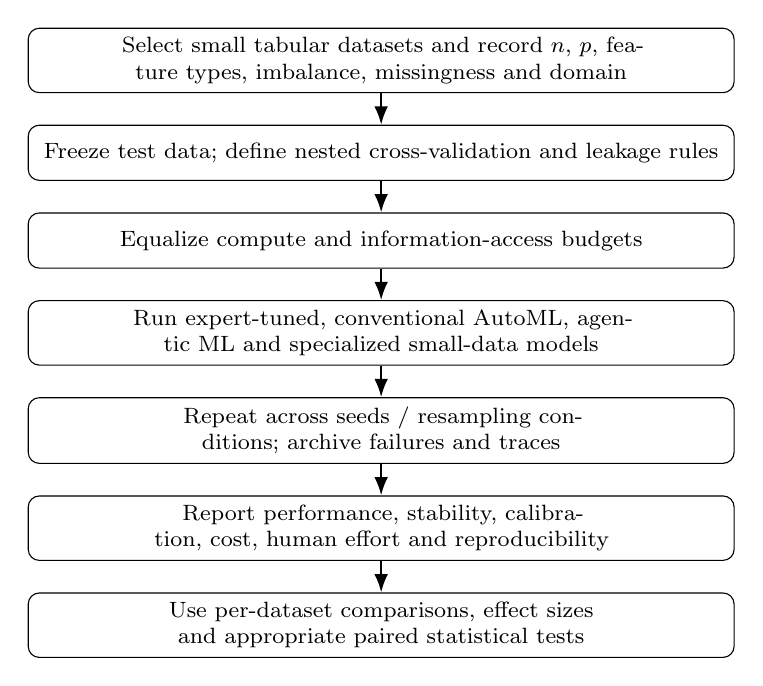
\begin{tikzpicture}[
node distance=4mm,
box/.style={draw, rounded corners, align=center, font=\footnotesize, minimum height=7mm, text width=0.72\linewidth},
arrow/.style={-Latex, thick}
]
\node[box] (datasets) {Select small tabular datasets and record $n$, $p$, feature types, imbalance, missingness and domain};
\node[box, below=of datasets] (split) {Freeze test data; define nested cross-validation and leakage rules};
\node[box, below=of split] (budget) {Equalize compute and information-access budgets};
\node[box, below=of budget] (methods) {Run expert-tuned, conventional AutoML, agentic ML and specialized small-data models};
\node[box, below=of methods] (repeat) {Repeat across seeds / resampling conditions; archive failures and traces};
\node[box, below=of repeat] (metrics) {Report performance, stability, calibration, cost, human effort and reproducibility};
\node[box, below=of metrics] (analysis) {Use per-dataset comparisons, effect sizes and appropriate paired statistical tests};
\draw[arrow] (datasets)--(split);
\draw[arrow] (split)--(budget);
\draw[arrow] (budget)--(methods);
\draw[arrow] (methods)--(repeat);
\draw[arrow] (repeat)--(metrics);
\draw[arrow] (metrics)--(analysis);
\end{tikzpicture}
\caption{Proposed controlled benchmarking workflow derived from the reviewed methodological gaps.}
\label{fig:protocol}
\Description{A sequential benchmark workflow from dataset characterization through nested validation, equal budgets, four model families, repeated runs, multidimensional metrics, and statistical analysis.}
\end{figure}

Six controls are crucial to the suggested methodology. Dataset properties are established before to the start of trials, and assessment data is kept separate from model selection. Every approach has its own computational allowance and criteria for outside information. All four approach families are evaluated using the same validation boundaries, with many runs to capture variation. Finally, the analysis takes into account forecast quality, cost, calibration, failures, and human participation.

\begin{table*}[!ht]
\caption{Variables and safeguards for the proposed benchmark}
\label{tab:protocol}
\centering
\small
\begin{tabularx}{\textwidth}{@{}p{0.19\textwidth}p{0.28\textwidth}X@{}}
\toprule
Dimension & Proposed safeguard & Purpose\\
\midrule
Dataset & Record $n$, $p$, feature types, imbalance, missingness and domain & Makes differences between datasets visible\\
Validation & Nested cross-validation; test set hidden & Keeps tuning separate from final evaluation\\
Search budget & Fixed wall-clock or compute budget & Limits differences in available search time\\
Information access & Same external-information policy & Avoids unfair advantages from outside information\\
Randomness & Multiple seeds / resampling runs & Shows variation between runs\\
Human effort & Record setup, debugging, analysis and intervention time & Captures the work required from users\\
Agent trace & Store prompts, model version, tools and generated code where permitted & Allows decisions and failures to be examined\\
Metrics & Performance, stability, calibration, cost and failure rate & Shows trade-offs beyond prediction score\\
\bottomrule
\end{tabularx}
\end{table*}

\section{Discussion}\label{sec:discussion}

The examined research do not show that expert tuning, traditional AutoML, agentic systems, or specialised small-data models are consistently superior in all situations.

An expert can tailor modelling choices to the dataset, but has limited time and may prefer known procedures. Conventional AutoML searches a bigger set of predefined alternatives, but its outcomes are dependent on the available search space and the reliability of validation scores. LLM agents can change the workflow itself, but their results vary between runs and are difficult to replicate. Pretrained small-data models move much of the learning work to an earlier stage; their success on a new dataset is dependent on whether that prior knowledge transfers.

A small improvement in accuracy may have limited practical value if it requires much more computation, human debugging, or API spending. In some applications, a slightly lower average score may be acceptable if the method is faster and produces more consistent results across resampling conditions.

For this reason, future comparisons would be more informative if they reported a range of outcomes instead of declaring one overall winner. Dataset-level scores should be accompanied by variation, calibration, failed runs, compute usage, and human effort. Mean rank can provide a compact overview:
\begin{equation}
\bar r_j=\frac{1}{N}\sum_{i=1}^{N}r_{ij},
\label{eq:rank}
\end{equation}
but the differences behind that average still need to be examined.

\section{Future Research Directions}\label{sec:future}

\subsection{Human-in-the-Loop AutoML}

Complete automation is not necessarily the most useful goal. One possibility is to combine the judgment of a human practitioner with automated planning and search. In a Human $\rightarrow$ Agent $\rightarrow$ AutoML $\rightarrow$ Human workflow, the expert could set constraints and review the outcome, while the agent and AutoML tools carry out much of the intermediate experimentation.

\subsection{Meta-Learning for Small Datasets}

Information gained from earlier small-data problems could help an AutoML system choose promising configurations before beginning a new search. Such meta-learning may be particularly useful when similar datasets are encountered repeatedly, since the system would not need to explore every choice from the beginning.

\subsection{Agentic Statistical Validation}

Creating functioning code is merely one of the requirements for agentic ML to be dependable. Agents also require more robust checks for data leakage, small or unrepresentative validation samples, unstable scores, class imbalance, selection bias, repeated testing, and inadequate probability calibration. These checks could become part of the experimental procedure rather than relying just on a final human assessment.

\subsection{Confidence-Aware Automation}

A model recommendation is easier to evaluate when it explains its uncertainty and practical cost. Future systems could display expected prediction quality, variability between runs, resource consumption, likely failure scenarios, and the reasoning for choosing that model, in addition to the pipeline.

\subsection{Anytime Benchmarking}

A single final-time result only provides a partial picture of search efficiency. Comparing approaches after 1, 5, 15, 60, and 240 minutes, for example, would reveal when good predictions become available and how much further improvement is possible with extra time. Work on Hyperband, BOHB, and FLAML encourages budget-sensitive evaluation \cite{li2018,falkner2018,wang2021}.

\section{Conclusion}\label{sec:conclusion}

AutoML has reduced the amount of manual work required to select algorithms, tweak hyperparameters, prepare data, and generate ensembles. The methodologies discussed here include Bayesian optimisation, genetic programming, bandit-based allocation, and methods designed to function within tight resource restrictions \cite{Feurer2015, Olson2016, Li2018, Falkner2018, Wang2021}. At the same time, AMLB demonstrates that judgements about competing frameworks can alter depending on the benchmark design and reporting outcomes \cite{gijsbers2024}.

Limited training data complicates matters further: validation estimates can be noisy, so a wider search does not always result in a more trustworthy model. TabPFN provides an alternative that relies on pre-trained knowledge instead of substantial tuning on each dataset \cite{hollmann2023}. LLM-based agents offer further possibilities by designing experiments, developing and running code, inspecting outcomes, and changing processes \cite{trirat2025}.

Taken together, the evidence suggests that these approaches should be evaluated for more than just predicted accuracy. The suggested benchmark thus emphasises validation design, comparable resource restrictions, information access, data leakage, randomisation, and human intervention. It also tracks calibration, stability, cost, reproducibility, and failures.

\section*{Acknowledgments}
This manuscript was prepared as part of the AI Tools for Research course assignment for Topic 27. The manuscript is based on the previously assigned research paper and its cited literature. No new empirical results are claimed.

\bibliographystyle{ACM-Reference-Format}
\bibliography{references}
\end{document}
